\documentclass[twocolumn]{bmcart}
%\setlength{\footskip}{30pt}

%% Use the option review to obtain double line spacing
%% \documentclass[authoryear,preprint,review,12pt]{elsarticle}

%% Use the options 1p,twocolumn; 3p; 3p,twocolumn; 5p; or 5p,twocolumn
%% for a journal layout:
%% \documentclass[final,1p,times]{elsarticle}
%% \documentclass[final,1p,times,twocolumn]{elsarticle}
%% \documentclass[final,3p,times]{elsarticle}
%% \documentclass[final,3p,times,twocolumn]{elsarticle}
%% \documentclass[final,5p,times]{elsarticle}
%% \documentclass[final,5p,times,twocolumn]{elsarticle}

%% For including figures, graphicx.sty has been loaded in
%% elsarticle.cls. If you prefer to use the old commands
%% please give \usepackage{epsfig}

\usepackage[utf8]{inputenc}
%\usepackage[T1]{fontenc}
%\usepackage{lmodern}
%\usepackage{tgpagella}

% Extensive support for hypertext.
\usepackage[hidelinks,colorlinks=true]{hyperref}

% Named references.
\usepackage{nameref}

% Easy access to the Lorem Ipsum dummy text.
\usepackage{lipsum}

% Pro­vides both fore­ground (text, rules, etc.) and back­ground colour man­age­ment.
%\usepackage{color}

% Driver-independent color extensions.
%\usepackage[x11names]{xcolor}

% Enhanced support for graphics.
\usepackage{graphicx}

% Produces figures which text can flow around.
\usepackage{wrapfig}

% Customising captions in floating environments.
%\usepackage{caption}

% Publication quality tables.
\usepackage{booktabs}

% Long tables.
\usepackage{longtable}

%% The amssymb package provides various useful mathematical symbols.
%\usepackage{amssymb}

%% The amsthm package provides extended theorem environments.
%\usepackage{amsthm}

%%%%%%%%%%%%%%%%%%%%%%%%%%%%%%%%%%%%%%%%%%%%%%%%%
%%                                             %%
%%  If you wish to display your graphics for   %%
%%  your own use using includegraphic or       %%
%%  includegraphics, then comment out the      %%
%%  following two lines of code.               %%
%%  NB: These line *must* be included when     %%
%%  submitting to BMC.                         %%
%%  All figure files must be submitted as      %%
%%  separate graphics through the BMC          %%
%%  submission process, not included in the    %%
%%  submitted article.                         %%
%%                                             %%
%%%%%%%%%%%%%%%%%%%%%%%%%%%%%%%%%%%%%%%%%%%%%%%%%

%\def\includegraphic{}
%\def\includegraphics{}

% Configure caption display.
%\captionsetup{margin=10pt,font=small,labelfont=bf,labelsep=period}

% Define where the images can be found.
\DeclareGraphicsExtensions{.pdf,.png,.jpg}
\graphicspath{{./images/}}

%%% Put your definitions there:
\startlocaldefs
\input{db-stats.inc}
\endlocaldefs

\begin{document}

% Configure hyperlink colors after document start to override possible
% documentclass defaults.
\hypersetup{
    citecolor=blue,
    filecolor=blue,
    linkcolor=blue,
    urlcolor=blue
}

\begin{frontmatter}

\begin{fmbox}
\dochead{Software}

%%%%%%%%%%%%%%%%%%%%%%%%%%%%%%%%%%%%%%%%%%%%%%
%%                                          %%
%% Enter the title of your article here     %%
%%                                          %%
%%%%%%%%%%%%%%%%%%%%%%%%%%%%%%%%%%%%%%%%%%%%%%

\title{Automated identification of slipper orchids using image analysis and artificial neural networks}

%%%%%%%%%%%%%%%%%%%%%%%%%%%%%%%%%%%%%%%%%%%%%%
%%                                          %%
%% Enter the authors here                   %%
%%                                          %%
%% Specify information, if available,       %%
%% in the form:                             %%
%%   <key>={<id1>,<id2>}                    %%
%%   <key>=                                 %%
%% Comment or delete the keys which are     %%
%% not used. Repeat \author command as much %%
%% as required.                             %%
%%                                          %%
%%%%%%%%%%%%%%%%%%%%%%%%%%%%%%%%%%%%%%%%%%%%%%

\author[
   addressref={nbc},
   %corref={},
   %noteref={},
   %email={}
]{\inits{S}\fnm{Serrano} \snm{Pereira}}
\author[
   addressref={nbc,hsl,lu},
   %corref={},
   noteref={n1},
   %email={}
]{\inits{B}\fnm{Barbara} \snm{Gravendeel}}
\author[
   addressref={nbc},
   %corref={},
   %noteref={},
   %email={}
]{\inits{P}\fnm{Patrick} \snm{Wijntjes}}
\author[
   addressref={nbc},
   %corref={},
   %noteref={},
   %email={}
]{\inits{R}\fnm{Rutger} \snm{Vos}}

% Dave Roberts co-author?

%%%%%%%%%%%%%%%%%%%%%%%%%%%%%%%%%%%%%%%%%%%%%%
%%                                          %%
%% Enter the authors' addresses here        %%
%%                                          %%
%% Repeat \address commands as much as      %%
%% required.                                %%
%%                                          %%
%%%%%%%%%%%%%%%%%%%%%%%%%%%%%%%%%%%%%%%%%%%%%%

\address[id=nbc]{
  \orgname{Naturalis Biodiversity Center}
  %\street{},
  %\postcode{}
  \city{Leiden},
  \cny{The Netherlands}
}

\address[id=hsl]{
  \orgname{University of Applied Sciences Leiden,}
  %\street{},
  %\postcode{}
  \city{Leiden},
  \cny{The Netherlands}
}

\address[id=lu]{
  \orgname{Institute Biology Leiden, Leiden University}
  %\street{},
  %\postcode{}
  \city{Leiden},
  \cny{The Netherlands}
}

%%%%%%%%%%%%%%%%%%%%%%%%%%%%%%%%%%%%%%%%%%%%%%
%%                                          %%
%% Enter short notes here                   %%
%%                                          %%
%% Short notes will be after addresses      %%
%% on first page.                           %%
%%                                          %%
%%%%%%%%%%%%%%%%%%%%%%%%%%%%%%%%%%%%%%%%%%%%%%

\begin{artnotes}
\note[id=n1]{Equal contributor} % note, connected to author
\end{artnotes}

% comment this for two column layout
%\end{fmbox}

%%%%%%%%%%%%%%%%%%%%%%%%%%%%%%%%%%%%%%%%%%%%%%
%%                                          %%
%% The Abstract begins here                 %%
%%                                          %%
%% Please refer to the Instructions for     %%
%% authors on http://www.biomedcentral.com  %%
%% and include the section headings         %%
%% accordingly for your article type.       %%
%%                                          %%
%%%%%%%%%%%%%%%%%%%%%%%%%%%%%%%%%%%%%%%%%%%%%%

\begin{abstractbox}

\begin{abstract}
A generic hierarchical identification system was developed for the automated identification of species by image recognition. The effectiveness of this system was assessed using photographs of orchids of the subfamily Cypripedioideae. Colour and shape features were extracted from single flower photos of {\SpeciesCount} orchid species. Generic image preprocessing, segmentation, and feature extraction algorithms were implemented to obtain morphometric data for the different orchid species. The identification system uses a hierarchy of artificial neural networks for pattern recognition and automated classification. The neural network hierarchy mirrors the taxonomic hierarchy of the Cypripedioideae, such that user-submitted photos could be assigned a genus, section, and species classification. The ability of the identification system to correctly identify user-submitted photos varied depending on the photo quality, the number of species included for training, and the desired taxonomic level for identification. High quality photos were scarce for some taxa and were under-represented in the training set, resulting in imbalanced network training. The simple colour features used for training were not sufficient to reliably identify photos to the correct section and species, and more specialised feature extraction algorithms need to be developed to improve accuracy. The outcomes of this project include an open source library of feature extraction libraries called ImgPheno, a collection of scripts for neural network training called NBClassify, and a web-interface for NBClassify called OrchiD for identification of user-submitted images.
\end{abstract}

%%%%%%%%%%%%%%%%%%%%%%%%%%%%%%%%%%%%%%%%%%%%%%
%%                                          %%
%% The keywords begin here                  %%
%%                                          %%
%% Put each keyword in separate \kwd{}.     %%
%%                                          %%
%%%%%%%%%%%%%%%%%%%%%%%%%%%%%%%%%%%%%%%%%%%%%%

\begin{keyword}
    \kwd{Cypripedioideae}
    \kwd{feature extraction}
    \kwd{identification}
    \kwd{image analysis}
    \kwd{neural networks}
    \kwd{orchids}
    \kwd{pattern recognition}
    \kwd{taxonomy}
\end{keyword}

% MSC classifications codes, if any
%\begin{keyword}[class=AMS]
%\kwd[Primary ]{}
%\kwd{}
%\kwd[; secondary ]{}
%\end{keyword}

\end{abstractbox}

% uncomment this for twcolumn layout
\end{fmbox}

\end{frontmatter}

%%%%%%%%%%%%%%%%%%%%%%%%%%%%%%%%%%%%%%%%%%%%%%
%%                                          %%
%% The Main Body begins here                %%
%%                                          %%
%% Please refer to the instructions for     %%
%% authors on:                              %%
%% http://www.biomedcentral.com/info/authors%%
%% and include the section headings         %%
%% accordingly for your article type.       %%
%%                                          %%
%% See the Results and Discussion section   %%
%% for details on how to create sub-sections%%
%%                                          %%
%% use \cite{...} to cite references        %%
%%  \cite{koon} and                         %%
%%  \cite{oreg,khar,zvai,xjon,schn,pond}    %%
%%  \nocite{smith,marg,hunn,advi,koha,mouse}%%
%%                                          %%
%%%%%%%%%%%%%%%%%%%%%%%%%%%%%%%%%%%%%%%%%%%%%%

\section{Introduction}
\label{sec:introduction}

Correct taxonomic identification of life is for different reasons of great importance. Considering the case of the Cypripedioideae, a horticultural popular group of orchids species and from which many species are highly endangered in the wild, correct taxonomic identification is necessary in order to protect them. Expert taxonomic identification is rare and costly, so alternative methods for taxonomic identification that are both cheap and accurate enough would be of great value. Ongoing advances in computer vision and machine learning has lead to the development of numerous semi- and fully automated species identification systems. Such systems have been successful in the identification of plant species \cite{Arinkin2014, Nilsback2008, Sanz2013}, phytoplankton \cite{Boddy1994}, diatom frustules \cite{Kloster2014}, and insects \cite{Weeks1999,Kang2012}, amongst others. Artificial Neural Networks (ANNs) in particular have become an increasingly popular choice in automated image classification systems \cite{Weeks1997}. They provide a powerful tool for pattern recognition and machine learning.

\section{Materials and methods}
\label{sec:methods}

% Used social media (crowd sourcing) for the collection of images.

\subsection{Reference photo collection}

In order to enable orchid identification through artificial neural networks means that neural networks must first be trained with a sufficient amount of photographs. A collection of reference photos was compiled by searching the internet for images, mostly through Google Image searches. Images were obtained from several multimedia resources like Flickr (\url{https://www.flickr.com}) and Wikimedia Commons (\url{http://commons.wikimedia.org}), but also from several orchid related websites (see \nameref{sec:acknowledgements}).

Simple strategies are needed for maintaining a large collection of reference images and their classification labels. An ideal solution would be a central server where images are stored along with their meta-data (i.e. taxonomic information required for training the neural networks). Such a database needs to be accessible via an application programming interface (API) which would allow for the implementation of custom image harvesters for easy retrieval of images and their meta-data. Secondly, such a database would need to be accessible from the internet so that images and meta-data could be maintained collaboratively via the internet.

The online image hosting service Flickr was used since it meets these requirements. Every photo was uploaded to an account on Flickr, where each image was annotated with standardized tags in the formats \verb/genus:name/, \verb/section:name/, and \verb/species:name/. The correct genus, section, and species for each image was verified by specialists and referenced to the literature \cite{Cribb1998, Pridgeon1999, Frosch2012} and phylogenetic reconstructions based on molecular analyses \cite{Li2011, Chochai2012}. A custom Python script utilising the Flickr API was implemented to mirror the reference images and associated meta-data on a local hard-drive prior image analysis. Images are stored in a directory hierarchy such that the directory names correspond to the image classes. Images are placed in subdirectories to correspond to their phylogenetic classifications. A local meta-data database (\ref{sec:meta-database}) is created for each reference image directory to enable querying of contained images, which is needed in downstream image processing.

\subsection{Image feature extraction}

Since raw pixel data are usually not appropriate for pattern recognition algorithms, images need to be summarised to one or more numerical values. These values, often called features, describe some aspect of the image contents. The algorithms or applications that compute these features are often called feature descriptors or feature extractors. Many feature extraction algorithms are generic and are not limited to specific images. Feature extractors can be applied to entire images and sometimes to regions of interest (ROI) in images. Many feature extraction algorithms exist and are described in the literature, and some have been implemented in software or software libraries for use in other software. Image recognition software that use pattern recognition and machine learning usually implement one or more feature extraction algorithms to summarize features and use those to train classifiers. With so many different feature extraction algorithms in the wild and new ones emerging periodically, finding the right algorithm for a specific image processing problem can be a daunting task, let alone having to implement such algorithms yourself if no existing implementation is readily available. Open Source Computer Vision (OpenCV) and Open Intelligent Multimedia Analysis for Java (OpenIMAJ) are comprehensive computer vision libraries that come with computer vision and machine learning algorithms (amongst others), but support for feature descriptors is currently limited. One of our goals was to implement a comprehensive and open-source software library of image feature description algorithms for the Python programming language, similar to what JFeatureLib does for Java. A proof-of-concept Python package called ImgPheno (\url{https://github.com/naturalis/imgpheno}) was developed during this study, which is not at all comprehensive in its current early development stage.

ImgPheno was implemented by a collection of proof-of-concept Python scripts (\url{https://github.com/naturalis/nbclassify}) for testing image recognition using hierarchical training of artificial neural networks. The scripts make extensive use of OpenCV \cite{Pulli2012} for computer vision, NumPy \cite{VanderWalt2011} for array manipulation, and of scikit-learn \cite{Pedregosa2011} for data transformation and cross-validation. Feature extraction and neural network training was automated with a custom Python script found in the NBClassify package. Configurations are kept in a separate YAML file so that neural network training can easily be reproduced. Different aspects of the feature extraction process can be configured with this configuration file: input/output format, data scaling, colour correction, foreground segmentation, feature descriptors to use, and a classification hierarchy definition for hierarchical training.

As part of the feature extraction workflow, each image is first scaled down if the image exceeds a predefined maximum dimension. This is followed by foreground segmentation to get the region of interest (ROI) matching the flower. Foreground segmentation is done with an iterative approach using the GrabCut segmentation algorithm \cite{Rother2004}. The ROI for the first iteration is set to the entire image and is shrank a fixed number of pixels to get a margin around the ROI containing obvious background pixels (figure \ref{fig:grabcut-output}). Images must therefore be reasonably standardized such that the flower is within this initial ROI. There must also be good contrast between the flower and the background, as to keep segmentation errors to a minimum. Subsequent iterations further classify pixels inside the ROI as foreground or background until the maximum number of iterations is reached. Contours are then obtained from the resulting binary mask, a copy of the image where foreground pixels are made white and background pixels black. Sometimes multiple contours are found (e.g. on images with multiple flowers) in which case only the largest contour is used to select the foreground pixels for downstream feature extraction.

\begin{figure*}[t]
    \centering
    \minipage{\textwidth}
        \includegraphics[width=0.48\linewidth]{grabcut_output_roi.png}
        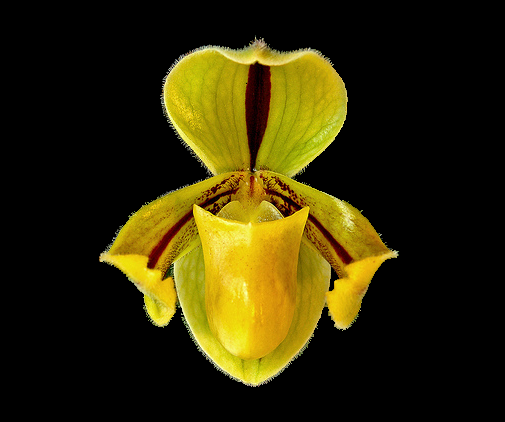
\includegraphics[width=0.48\linewidth]{grabcut_output.png}
    \endminipage
    \caption{Foreground segmentation with the GrabCut algorithm. The image on the left displays how the initial region of interest is set during automated feature extraction. Photo of \textit{Paphiopedilum druryi} by Peter Tremain.}
    \label{fig:grabcut-output}
\end{figure*}

Only one feature extractor was used to extract features for subsequent training of the artificial neural networks. This feature extractor computes summarised histograms from the pixel colour intensities for the BGR colour space. This was done by calculating the up-right bounding square for the main contour, dividing the square into $N$ equal horizontal and vertical sections (bins), and calculating the mean blue, green, and red colour intensity for each bin. This results in two histograms, one for the horizontal and one for the vertical bins (figure~\ref{fig:bgr-means-sections}). Plotting the histograms shows that this feature captures some aspect of flower shape as well (figure~\ref{fig:bgr-means-plots}).

\begin{figure}[h]
    \centering
    \includegraphics[width=0.46\textwidth]{bgr_means_sections.png}
    \caption{The second horizontal and vertical bin ($N~=~20$) is highlighted in a foreground segmented image of \textit{P.~druryi}.}
    \label{fig:bgr-means-sections}
\end{figure}

\begin{figure*}[t]
    \centering
    \includegraphics[width=\textwidth]{bgr_means_plots.pdf}
    \caption{Plots of the mean BGR colour intensities for an image of \textit{P. druryi}. The plots display the mean intensities for the horizontal and vertical bins respectively.}
    \label{fig:bgr-means-plots}
\end{figure*}

\subsection{Neural network training}

Because the 140+ species of the subfamily Cypripedioideae poses a challenge for training a single neural network, a hierarchical approach was used. Hierarchical multi-species classification was done with a hierarchical system of feedforward artificial neural networks that was trained using the iRPROP backpropagation training algorithm. Artificial neural network (ANN) training was implemented with the Fast Artificial Neural Network Library (FANN) by \cite{Nissen2003}. Hierarchical training results in multiple neural networks: one ANN for genus classification, one ANN per genus for section classification, and one ANN per section for species classification. For the individual neural networks this means they need to differentiate between fewer classes and they can be trained using rank or taxon specific features. No ANNs need to be trained on nodes where no branching occurs in the hierarchy (e.g. unispecific genera). Hierarchical classification also means that an incorrect classification at a higher rank in the hierarchy results in incorrect subsequent classifications at lower ranks. It also allows for partial classifications when classification fails for the lower ranks.

The classification hierarchy is defined in the configurations file and is defined as a list of levels for the classification hierarchy which tells the training script the path to follow during training and classification. In this study the levels were named after the corresponding taxonomic ranks: $genus \rightarrow section \rightarrow species$. Different features and training parameters can be set at each level in the classification hierarchy, which the script then uses to generate training data for the required ANNs. All training data was scaled to a -1 to 1 range as per the span of the used activation function (symmetric sigmoid). Codewords were used to encode the class for each sample in the training data. Each ANN has its own set of codewords generated from the sorted lists of classes the ANN is trained on. Each codeword consists of $N$ bits, where $N$ is the number of classes the ANN is trained on. All bits in the codeword are set to an off value (-1), except for one bit (1) which corresponds to the class in the sorted list of classes. Once the training data is generated they are used to train the individual neural networks.

FANN supports many training parameters (e.g. training algorithms, activation functions, neural network topology, etc.) and since there is no way of telling which parameters and which combination of algorithms work best for a specific classification problem, tuning of parameters becomes a matter of trial-and-error. A framework for evolving optimal neural networks (\verb/AI::FANN::Evolving/, \url{https://github.com/naturalis/ai-fann-evolving}) was implemented to overcome this issue. The library implements a genetic algorithm to automate the trial-and-error process with different training parameters, which results in a single ``fittest'' neural network.

\subsection{Cross-validation}

Stratified k-folds cross-validation was performed to estimate the accuracy of hierarchical classification. Genus-section-species combinations were used as the classes for the cross-validations. Because the amount of images for some taxa were very limited, taxa for which the number of images was less than the number of folds ($k$) were excluded. Cross-validation was performed with both standard training and training via the genetic algorithm.

Principal components analysis (PCA) was performed on the training data to assess the suitability of the features for differentiating the photos by genus, section, and species. PCA with orthogonal rotation (varimax) was conducted on several training data sets containing -1 to 1 scaled mean colour intensities for the BGR colour space with 20 horizontal and vertical bins, which translates to 120 features. The Kaiser-Meyer-Olkin measure was used to verify the sampling adequacy for the analysis. Bartlett's test of sphericity was used to get indications whether correlations between items were sufficiently large for PCA. The inflexion in scree plots were used to set the number of components to be extracted. PCA was performed on training data for genus classification, section classification within the genus \textit{Paphiopedilum}, and for species classification within the section \textit{Parvisepalum} of genus \textit{Paphiopedilum}. PCA was not performed for the remaining data sets because the number of features often exceeds the sample size.

\section{Results}
\label{sec:results}

\subsection{Reference photo collection}

In total {\PhotoCount} photos for {\SpeciesCount} species were collected from various sources (table~\ref{tbl:photo-counts}). The collection represents all five genera from subfamily Cypripedioideae: \textit{Cypripedium}, \textit{Mexipedium}, \textit{Paphiopedilum}, \textit{Phragmipedium}, and \textit{Selenipedium}. With the number of photos for the five genera ranging from just 4 for the genus \textit{Selenipedium} to 888 for \textit{Paphiopedilum}, the collection is highly unbalanced. There is also a high variation in the number of images within genera. Unbalanced data results in a bias towards the more image rich taxa during neural network training, meaning the under-represented taxa are less likely to be classified correctly.

Because images of some taxa were hard to find, we had to make some compromises with respect to the quality of the images. Many of the gathered images are not of the desired standardised format, resulting in variations in background, lighting, dimension, and flower position or rotation, which makes pattern recognition more challenging. Since foreground segmentation is part of the automated workflow, this sometimes results in incorrectly segmented images.

The complete reference set can be found on Flickr: \url{https://www.flickr.com/photos/113733456@N06/}. Reference images can be downloaded in batch and placed in a directory hierarchy using the \verb/nbc-harvest-images/ script of the NBClassify package. Alternatively, the \verb/nbc-trainer/ script can be used to create a meta-data database from an existing image directory, which would enable subsequent training on images of that directory.

\begin{table}[h]\footnotesize
    \caption{The number of photos collected per genus, as well as the number of sections and species per genus represented by the photo collection.}
    \begin{center}
    \begin{tabular}{llll}
    \toprule
    \textbf{Genus} & \textbf{Section} & \textbf{Species} & \textbf{Photos} \\
    \midrule
    \input{table-taxa-summary.inc}
    \bottomrule
    \end{tabular}
    \end{center}
    \label{tbl:photo-counts}
\end{table}

\subsection{Image feature extraction}

The ImgPheno library is currently at an early development stage and only a few feature extraction algorithms have been implemented so far. The library also includes a few reference implementations of colour enhancement algorithms, helper functions for feature drawing, and algorithms that implement image features to compute shape properties (e.g. computing the centre point from moments). An overview of the descriptors and enhancement functions can be found in table~\ref{tbl:imgpheno-methods}.

\begin{table}[h]\footnotesize
    \caption{ImgPheno features and methods overview.}
    \begin{center}
    \begin{tabular}{p{3.5cm}p{3.5cm}}
    \toprule
    \textbf{Method} & \textbf{Description} \\
    \midrule
    Colour Histogram & Returns the histogram for an image. \\
    Binned Colour Histogram & Returns histograms for the mean BGR intensities from the horizontally and vertically segmented image. \\
    Contour Eccentricity & Computes a scalar that specifies the eccentricity of the ellipse that fits the contour. The eccentricity is the ratio of the distance between the centre and either focus of the ellipse and its major axis length. \\
    Contour Equivalent Diameter & Computes a scalar that specifies the diameter of a circle with the same area as the contour. \\
    Contour Solidity & Computes a scalar specifying the proportion of the pixels in the convex hull that are also in the region. \\
    Contour Outline & Computes a vector that summarizes the outlines of a contour at a specified resolution. \\
    Contour Centre Based Branch Lengths & Computes a vector that summarizes the outline of a contour using branch lengths from the centre of mass. \\
    \midrule
    Linear Colour Enhancement & Provides a hue preserving linear transformation with maximum possible contrast \cite{Naik2003}. \\
    Non-linear Colour Enhancement & Provides non-linear hue preserving transformation without gamut problem, provided that linear transformation is initially applied on each of the pixels \cite{Naik2003}. \\
    S-type enhancement function & This implements the S-type enhancement function for contrast enhancement of grey scale images \cite{Naik2003}. Can be used as the enhancement function for non-linear colour enhancement. \\
    \bottomrule
    \end{tabular}
    \end{center}
    \label{tbl:imgpheno-methods}
\end{table}

\subsection{Cross-validation}

Stratified k-folds cross-validation was performed to estimate the accuracy of hierarchical classification. The accuracy for genus classification was 75\%, but accuracy drops dramatically as section (52\%) and species (48\%) are also included in the classification (table~\ref{tbl:x-validation-results}). With 10 folds and including only those species for which at least 10 photos were collected, results in slightly better accuracies (table~\ref{tbl:x-validation-results}), which can probably be attributed to the reduced number of taxa and more equal image representation between taxa.

\begin{table}[h]\footnotesize
    \caption{Results for stratified k-fold cross-validations. Cross-validation was performed on three taxonomic ranks: genus, section, and species. The results for genus/section and genus/section/species combine the results from their respective ranks.}
    \begin{center}
    \begin{tabular}{lp{1.5cm}p{1.5cm}}
    \toprule
    \textbf{Classification} & \textbf{Accuracy (k=4)} & \textbf{Accuracy (k=10)} \\
    \midrule
    genus                   & 75\%    & 81\% \\
    section                 & 52\%    & 60\% \\
    species                 & 48\%    & 56\% \\
    genus/section           & 41\%    & 49\% \\
    genus/section/species   & 20\%    & 27\% \\
    \bottomrule
    \end{tabular}
    \end{center}
    \label{tbl:x-validation-results}
\end{table}

Figure~\ref{fig:pca-plots} shows the scatter plots for the principal component analyses (PCAs) that were performed on a subset of the training data. The poor classification accuracies described in table \ref{tbl:x-validation-results} may be attributed to the poor discrimination ability of the colour based feature to the different taxa and on improper foreground segmentation. Out of the four plots, only the plot for species classification within the section \textit{Parvisepalum} of genus \textit{Paphiopedilum} showed some clear clusters. The accuracy for species classification within this section was 85\% and 88\% for 4 and 10 folds respectively. This compares fairly well with genus classification, which is surprising when comparing the scatter plots for genus classification and \textit{Parvisepalum} species classification.

\subsection{OrchiD: slipper orchid identification of user-submitted images}

ImgPheno and NBClassify were implemented in a proof-of-concept web application ``OrchiD'' for the identification of slipper orchids from user-submitted images. This web application was developed as a Django application and is included in the NBClassify source repository.

\section{Conclusions and discussion}
\label{sec:conclusion}

From the cross-validations it is surprising to see that genus classification results in higher accuracies than section and species classification (75\% vs. 52\% vs. 48\%), since the ANNs for lower ranks only need to deal with a subset of the reference images. This may be explained by the fact that the ANN for genus classification has knowledge of all classes. Maybe the trick is to include all images in the train data, even for the ANNs of lower ranks, by adding a class ``other'' for images not belonging to the parent class.

In an effort the normalize images prior to feature extraction, some colour image enhancement methods developed by \cite{Naik2003} were implemented. Most images used were already of good quality, and performing hue-preserving linear transformation with maximum contrast often did not result in an enhanced image, and identification accuracy was not significantly improved.

As opposed to simply using colour histograms as described in this study, image feature extraction methods should also be developed for extracting specific morphological characters to improve accuracy with hierarchical classification. Developing such specialized features extraction methods is not an easy task however. Many different specialized image feature extraction methods have been developed, and it would be desirable to have these combined in a freely available library, as was attempted in this study. And since multiple morphological characters are usually considered during species identification, multiple features can be used for ANN training. Identification accuracy can further be improved by means of neural network ensembles where multiple neural networks are used to make classifications \cite{Hansen1990}. The identification system presented here does use multiple neural networks for the identification of an image, but these cannot be considered neural networks ensembles because only one neural network is used for each level within the hierarchical classification. The output codes used for training the neural networks as implemented in this study is another aspect that could be improved. The implementation presented here uses the simplest possible output codes for training, but the usage of more sophisticated error codes could improve neural network training and therefore identification accuracy \cite{Dietterich1995}.

The ImgPheno image feature extraction library is currently a mixture of feature descriptors, enhancement functions, helper functions for drawing features on images, clustering functions, and algorithms that implement such feature descriptors. For an image features library it would be more desirable to have only reference implementations for image features and image feature detectors. Algorithms that depend on image features should be developed separately from such a library. ImgPheno was developed in Python, but to make such a library interesting for high-throughput purposes, it would be better to develop such a library in a lower level programming language that can easily be interfaced to other programming languages (e.g. C++). It might even make more sense to extend existing computer vision libraries with said algorithms. OpenCV is an open-source library that already implements a range of image feature (detection) algorithms, and such a library could easily be contributed to with new algorithms. As a bonus it already comes with interfaces to many other programming languages.

% Need more and better photo material.
% Better feature extraction methods.

%%%%%%%%%%%%%%%%%%%%%%%%%%%%%%%%%%%%%%%%%%%%%%
%%                                          %%
%% Backmatter begins here                   %%
%%                                          %%
%%%%%%%%%%%%%%%%%%%%%%%%%%%%%%%%%%%%%%%%%%%%%%

\begin{backmatter}

\section*{Acknowledgements}
\label{sec:acknowledgements}

% De namen van alle fotografen in de format J.H. Simpson.

This research was made possible by the xxx grant. We are thankful to the following photographers and institutions for allowing us to use their photographs for this research: Alpine-Garden.com, Clark Riley, Crustacare, Dalton Holland Baptista, Daniel Winkler, Danuta Panczyk, David Llewelyn, Dot Potter Barnett, Eleanor S. Saulys (Connecticut Orchid Society), Eric Hunt, Eric Hunt, Fren Mah, GoreOrchids.com, Greentours, Holger Perner, J.J. Harrison, Jason Chang, Jean Claessens, John Marcotte, Joseph W. Dougherty, Karma Forester, Markus Bürki (Botanischer Garten Bern), Martin Günther, Mauro Rosim, Mihai Costea, Nile and Lois Dusdieker, Orchi, Patrick Mannens, Peter Tremain, Philipp J. Cribb and the Swiss Orchid Foundation, Pieter C. Brouwer, Pilar Quintana, Ray Barkalow (First Rays Orchids), Rene Klinge, Rick H., Richard Labbe (Planteck), Roberto Takase, Rogier van Vugt, Ron Parsons, Ross Hella, Vermont Ladyslipper Company, Yijia Wang, GoreOrchids.com, and Orchids.com.

%%%%%%%%%%%%%%%%%%%%%%%%%%%%%%%%%%%%%%%%%%%%%%%%%%%%%%%%%%%%%
%%                  The Bibliography                       %%
%%                                                         %%
%%  Bmc_mathpys.bst  will be used to                       %%
%%  create a .BBL file for submission.                     %%
%%  After submission of the .TEX file,                     %%
%%  you will be prompted to submit your .BBL file.         %%
%%                                                         %%
%%                                                         %%
%%  Note that the displayed Bibliography will not          %%
%%  necessarily be rendered by Latex exactly as specified  %%
%%  in the online Instructions for Authors.                %%
%%                                                         %%
%%%%%%%%%%%%%%%%%%%%%%%%%%%%%%%%%%%%%%%%%%%%%%%%%%%%%%%%%%%%%

% if your bibliography is in bibtex format, use those commands:
\bibliographystyle{bmc-mathphys} % Style BST file
%\bibliographystyle{apa}
%\biboptions{authoryear}

% or include bibliography directly:
% \begin{thebibliography}
% \bibitem{b1}
% \end{thebibliography}

\bibliography{report}

%% The Appendices part is started with the command \appendix;
%% appendix sections are then done as normal sections
\appendix
\onecolumn

\section{Metadata database}
\label{sec:meta-database}

\begin{figure*}[!h]
    \centering
    \includegraphics[width=\textwidth]{meta_database_diagram.pdf}
    \caption{Diagram of the metadata database used for storing taxonomic information for a collection of reference photos.}
    \label{fig:meta-database}
\end{figure*}

\section{Reference photo collection}
\label{sec:reference-photo-collection}

\begin{scriptsize}
\begin{longtable}{llllll}
    \caption{Taxa represented by the reference photo collection and the number of photos for each species.}
    \label{tbl:taxa-stats}
    \endfirsthead
        \caption*{\textbf{Table \ref{tbl:taxa-stats}.} (continued)}
        \\\textbf{Taxa} & \textbf{Photos} \\
        \midrule
    \endhead
        \midrule
        \caption*{\scriptsize\textit{(continued on next page)}}
    \endfoot
        \bottomrule
    \endlastfoot

    \toprule
    \textbf{Taxa} & \textbf{Photos} \\
    \midrule
    \input{table-taxa.inc}
\end{longtable}
\end{scriptsize}

\clearpage
\section{Scatter plots for principal components analyses}
\label{sec:pca-plots}

\begin{figure}[!h]
    \minipage{\textwidth}
        \includegraphics[width=0.5\linewidth]{genus_pca_plot.pdf}
        \includegraphics[width=0.5\linewidth]{Cypripedium_section_pca_plot.pdf}
    \endminipage
    \par\vfill
    \minipage{\textwidth}
        \includegraphics[width=0.5\linewidth]{Paphiopedilum_section_pca_plot.pdf}
        \includegraphics[width=0.5\linewidth]{Paphiopedilum_Parvisepalum_species_pca_plot.pdf}
    \endminipage
    \caption{Scatter plots for the principal components analysis results. PCA was conducted on training data for genus classification, \textit{Cypripedium} section classification, \textit{Paphiopedilum} section classification, and \textit{Paphiopedilum} section \textit{Parvisepalum} species classification. For all plots the first principal component (PC1) was plotted against the second (PC2).}
    \label{fig:pca-plots}
\end{figure}

\end{backmatter}
\end{document}
